\documentclass{article}

\usepackage[romanian]{babel}
\usepackage[a4paper]{geometry}
\usepackage{graphicx}
\usepackage[hidelinks]{hyperref}
\usepackage{microtype}

\graphicspath{ {../images/} }

\title{Sokoban\\Tema 1 - Inteligență Artificială}
\author{Alexandru Sima (332CA)}

\begin{document}

\maketitle
\begin{abstract}
    Analiza a 2 strategii de rezolvare a jocului de Sokoban prin explorarea 
    spațiului stărilor: \textbf{Beam Search} și \textbf{Learning Real-Time A*}. 
    Prezentarea unei soluții de rezolvare și evaluarea performanțelor, comparând
    cele 2 strategii, cât și prezentarea raționamentului care a condus la 
    această soluții și comparații cu idei anterioare.
\end{abstract}

\newpage
\tableofcontents

\newpage
\section{Soluție propusă}

\subsection{Beam Search}
Algoritmul funcționează după cum urmează: se pleacă de la o stare inițială,
care va reprezenta \textit{beam-ul} inițial; la fiecare pas, se expandează 
vecinii fiecărei stări din \textit{beam}, se elimină duplicatele și se 
calculează costul fiecărei stări, conform euristicii, apoi se aleg următoarele 
$k$ stări pentru a forma noul \textit{beam}. Pentru a evita anumite situații
în care algoritmul se blochează în niște minime locale ale funcției de cost, 
am ales o abordare stocastică: nu se aleg cele mai bune $k$ stări, ci $k$ stări 
cu o probabilitate care ia în calcul costul stării (aplicând 
softmax\footnote{\url{https://en.wikipedia.org/wiki/Softmax_function}} pe 
costurile obținute).

Algoritmul poate fi ajustat prin:
\begin{itemize}
    \item \textit{heuristic}: funcție care estimează costul unei stări;
    \item \textit{state\_generator}: funcție care generează vecinii unei stări;
    \item \textit{max\_iters}: numărul maxim de iterații ale \textit{beam-ului}
    până la care se încearcă rezolvarea;
    \item \textit{k}: dimensiunea \textit{beam-ului}.    
\end{itemize}

\subsection{Learning Real-Time A*}
Algoritmul, ca și cel precedent, pornește dintr-o stare inițială, și, la fiecare
pas, evaluează vecinii stării în care se află și avansează înspre cel de cost 
minim. Pentru a învăța costurile (și a converge spre costurile reale), se rețin 
într-o tabelă asocieri $(stare \rightarrow cost)$. Aceasta se populează cu 
valori când se evaluează o stare nemaiîntâlnită (se introduce costul estimat de 
euristică) și la fiecare tranziție între stări (fiind cel mai bun cost cunoscut,
se consideră că este mai aproape de adevăr). Deoarece, când nu este permis ca
jucătorul să tragă cutii, pot exista stări de deadlock (în care jocul este 
pierdut), dacă, după un număr stabilit de pași, algoritmul nu găsește o stare cu
un cost mai bun, acesta repornește din starea inițială (reținând tabela de 
estimări, pentru a o îmbunătăți mai departe).

Algoritmul poate fi ajustat prin:
\begin{itemize}
    \item \textit{heuristic}: funcție care estimează costul unei stări;
    \item \textit{state\_generator}: funcție care generează vecinii unei stări;
    \item \textit{max\_iters}: numărul maxim de mișcări din starea inițială până
    la care se încearcă rezolvarea;
    \item \textit{max\_restarts}: numărul maxim de resetări în starea inițială;
    \item \textit{steps\_before\_restart}: numărul de stări vizitate succesiv 
    fără găsirea unui cost mai bun la care se resetează algoritmul în starea 
    inițială.
\end{itemize}

\subsection{Euristica propusă}

Funcția de cost aleasă pentru algoritmii de căutare este suma distanțelor de la
cutii la pătrățelele țintă. Pentru fiecare cutie, se calculează distanța 
(în împingeri) către fiecare pătrățel de pe hartă (și, implicit, către fiecare 
țintă), apoi se asociază fiecărei cutii o țintă, astfel încât suma distanțelor 
să fie minimă. Împerechearea se face cu ajutorul 
\textit{Hungarian method}\footnote{\url{https://en.wikipedia.org/wiki/Hungarian_algorithm}}, 
implementată deja în \textit{Python} în biblioteca \textit{scipy} 
(\textit{scipy.optimize.linear\_sum\_assignment}).


\subsection{Analiza performanțelor}

Parametri utilizați:
\begin{itemize}
    \item Parametri comuni:
    \begin{itemize}
        \item \textit{heuristic}: Manhattan;
        \item \textit{state\_generator}: mutări fără trageri;
        \item \textit{max\_iters}: 200;
    \end{itemize}
    \item Beam Search:
    \begin{itemize}
        \item \textit{k}: 80;
    \end{itemize}
    \item Learning Real-Time A*:
    \begin{itemize}
        \item \textit{max\_restarts}: 500;
        \item \textit{steps\_before\_restart}: 50;
    \end{itemize}
\end{itemize}

Rulând algoritmii pe setul de teste furnizat, se observă următoarele tipare:

\subsubsection*{Timpul de execuție}
Timpul de execuție pentru algoritmul Beam Search este semnificativ mai mare
decât cel pentru Learning Real-Time A*, datorită nevoii de a evalua vecinii 
tuturor stărilor din beam la fiecare pas (\textit{lungime\_beam} $\cdot$ 
\textit{număr\_vecini} $\approx k \cdot 4$); LRTA*, pe de altă parte, consideră
doar starea curentă și vecinii acesteia. Se poate observa în (\ref{fig:time}) că
LRTA* este de $\approx 3$ ori mai rapid decât Beam Search pentru o bună parte 
din teste. 

\begin{figure}
    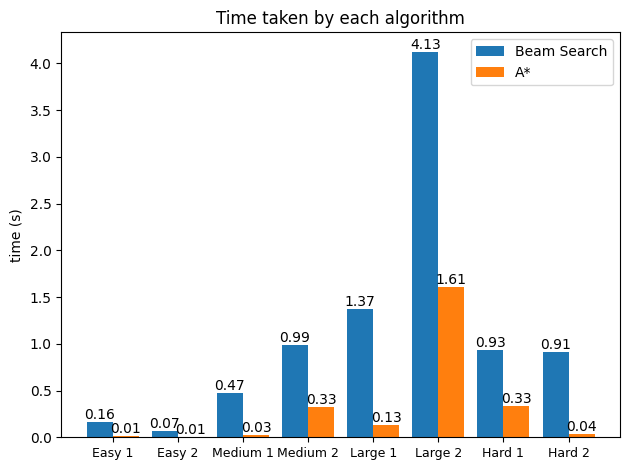
\includegraphics[scale=0.8]{plots/solution/time.png}
    \caption{Timpul de execuție al algoritmilor pe diferite teste}
    \label{fig:time}
\end{figure}

\subsubsection*{Numărul de stări vizitate}
Din aceleași considerente ca mai sus, numărul de stări vizitate (incluse în beam
în cazul Beam Search) este mai mic în cazul LRTA*, deoarece acesta consideră 
doar starea curentă. Diferența este însă mai mică, mai ales în cazul testelor 
complexe și cu multe "stări capcană", după cum se poate observa în 
(\ref{fig:states}), deoarece LRTA* trebuie să revină în starea inițială pentru
a evita \textit{deadlock}-urile.

\begin{figure}
    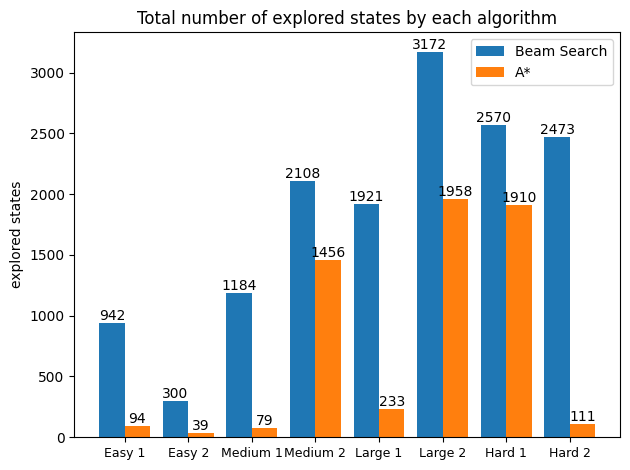
\includegraphics[scale=0.8]{plots/solution/states.png}
    \caption{Numărul de stări vizitate de algoritmi în cazul fiecărui test}
    \label{fig:states}
\end{figure}

\subsubsection*{Optimalitatea soluției}
Conform rezultatelor din (\ref{fig:solution_length}), Beam Search găsește 
soluții mai scurte decât LRTA*, deoarece cel din urmă poate să se întoarcă în 
stări anterioare pentru că învață în timp real costurile stărilor. Exploatând 
acest comportament, putem reporni algoritmul LRTA* de mai multe ori, ținând cont
de estimările anterioare de cost, pentru a găsi soluții mai bune, deoarece
algoritmul converge către costurile reale. Se poate vedea în 
(\ref{fig:enhanced_astar}) că se obțin soluții în general mai bune, dar, pentru
anumite teste, nu este suficient, chiar dacă se repornește de 100 de ori!

\begin{figure}
    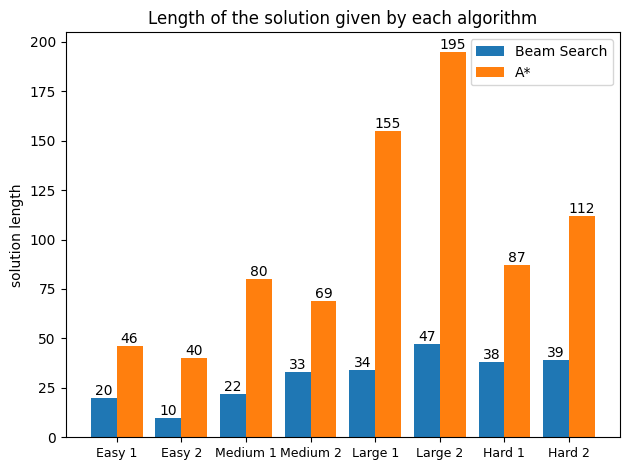
\includegraphics[scale=0.8]{plots/solution/solution_length.png}
    \caption{Lungimea soluției (numărul de mișcări) găsite de algoritmi pentru 
    teste}
    \label{fig:solution_length}
\end{figure}

\begin{figure}
    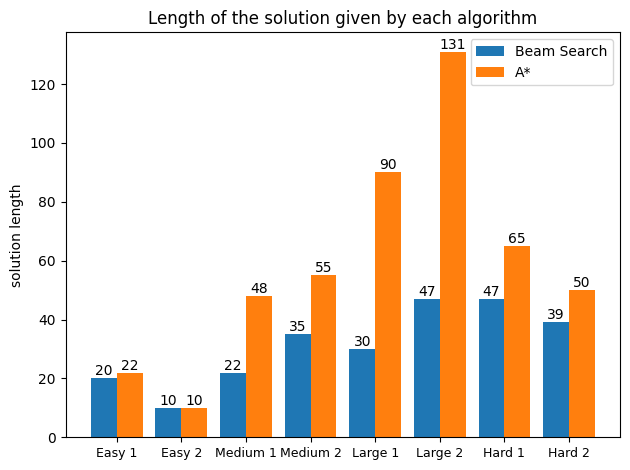
\includegraphics[scale=0.45]{plots/solution/enhanced_astar/solution_length.png}
    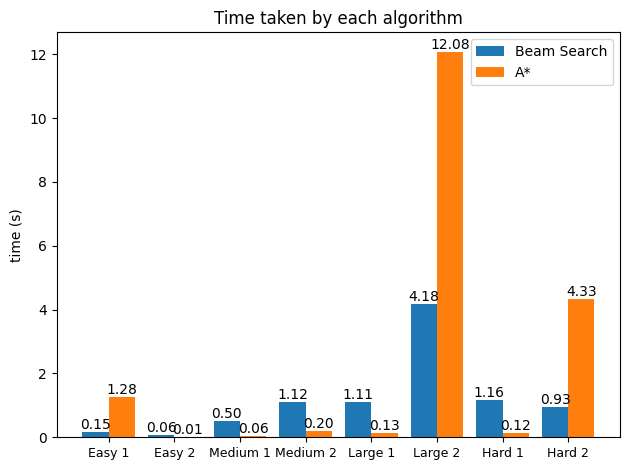
\includegraphics[scale=0.45]{plots/solution/enhanced_astar/time.png}
    \caption{Lungimile soluțiilor și durata execuției pentru Beam Search și 
    LRTA* cu 100 de reporniri după găsirea soluției}
    \label{fig:enhanced_astar}
\end{figure}

\section{Raționament}
% \section{Beam search}

% Am început prin a sorta starile in functie de distantele de la cutii la 
% obiective, apoi de la jucator la cutii (pentru a nu avea egalitate intre starile
% in care nu se muta o cutie). Nu s-a dovedit folositor nici macar pentru exemplul
% din schelet, deoarece se impingea cutia in perete (mai aproape - d.p.d.v al 
% distanței Manhattan - de obiectiv, apoi se bloca).
% \begin{figure}[ht]
%     % 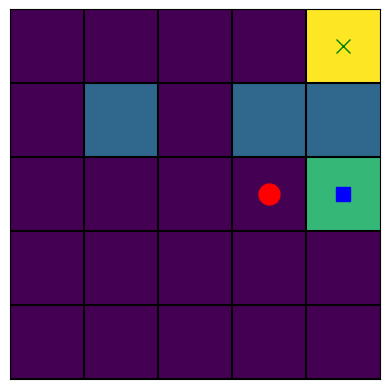
\includegraphics[scale=0.4]{a}
%     % 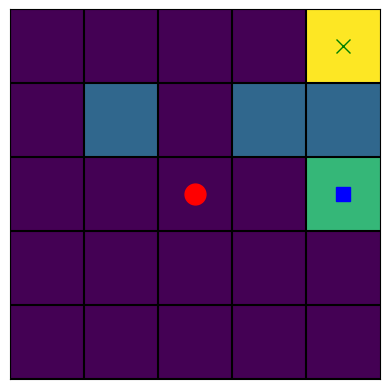
\includegraphics[scale=0.4]{b}
%     \caption{Primul impas: Cutia nu poate fi adusă la țintă fără a fi 
%     îndepărtată întâi de aceasta}
% \end{figure}

% O optimizare a evaluării stărilor a fost ca distanța cutiilor spre obiective să 
% nu mai fie calculata folosind distanta Manhattan, ci prin cel mai scurt drum 
% prin arenă de la cutie la o țintă. Cum țintele erau fixe, aceste distanțe se pot
% precalcula pentru eficientizare. Această nouă versiune ajungea în continuare 
% într-un impas, cand jucătorul trebuia sa se îndepărteze de o cutie pentru a o 
% muta din alt unghi.
% \begin{figure}[ht]
%     % 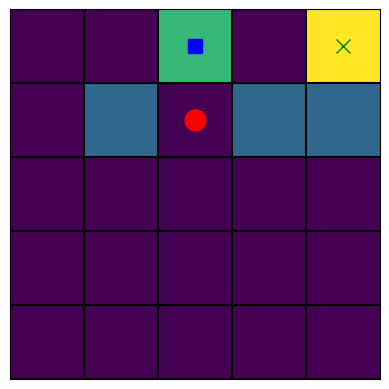
\includegraphics[scale=0.4]{a2}
%     % 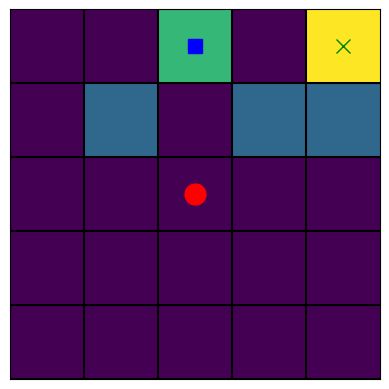
\includegraphics[scale=0.4]{b2}
%     \caption{Al 2-lea impas: Cutia nu poate fi mutată fără ca jucătorul să se 
%     îndepărteze de aceasta}
% \end{figure}

\end{document}